\documentclass[aspectratio=169]{../latex_main/tntbeamer}  % you can pass all options of the beamer class, e.g., 'handout' or 'aspectratio=43'
\usepackage{dsfont}
\usepackage{bm}
\usepackage[english]{babel}
\usepackage[T1]{fontenc}
%\usepackage[utf8]{inputenc}
\usepackage{graphicx}
\graphicspath{ {./figures/} }
\usepackage{algorithm}
\usepackage[ruled,vlined,algo2e,linesnumbered]{algorithm2e}
\usepackage{hyperref}
\usepackage{booktabs}
\usepackage{mathtools}

\usepackage{amsmath,amssymb}

\DeclareMathOperator*{\argmax}{arg\,max}
\DeclareMathOperator*{\argmin}{arg\,min}

\usepackage{amsbsy}
\newcommand{\vect}[1]{\bm{#1}}
%\newcommand{\vect}[1]{\boldsymbol{#1}}

\usepackage{pgfplots}
\pgfplotsset{compat=1.16}
\usepackage{tikz}
\usetikzlibrary{trees} 
\usetikzlibrary{shapes.geometric}
\usetikzlibrary{positioning,shapes,shadows,arrows,calc,mindmap}
\usetikzlibrary{positioning,fadings,through}
\usetikzlibrary{decorations.pathreplacing}
\usetikzlibrary{intersections}
\pgfdeclarelayer{background}
\pgfdeclarelayer{foreground}
\pgfsetlayers{background,main,foreground}
\tikzstyle{activity}=[rectangle, draw=black, rounded corners, text centered, text width=8em]
\tikzstyle{data}=[rectangle, draw=black, text centered, text width=8em]
\tikzstyle{myarrow}=[->, thick, draw=black]

% Define the layers to draw the diagram
\pgfdeclarelayer{background}
\pgfdeclarelayer{foreground}
\pgfsetlayers{background,main,foreground}

% Requires XeLaTeX or LuaLaTeX
%\usepackage{unicode-math}

\usepackage{fontspec}
%\setsansfont{Arial}
\setsansfont{RotisSansSerifStd}[ 
Path=../latex_main/fonts/,
Extension = .otf,
UprightFont = *-Regular,  % or *-Light
BoldFont = *-ExtraBold,  % or *-Bold
ItalicFont = *-Italic
]
\setmonofont{Cascadia Mono}[
Scale=0.8
]

% scale factor adapted; mathrm font added (Benjamin Spitschan @TNT, 2021-06-01)
%\setmathfont[Scale=1.05]{Libertinus Math}
%\setmathrm[Scale=1.05]{Libertinus Math}

% other available math fonts are (not exhaustive)
% Latin Modern Math
% XITS Math
% Libertinus Math
% Asana Math
% Fira Math
% TeX Gyre Pagella Math
% TeX Gyre Bonum Math
% TeX Gyre Schola Math
% TeX Gyre Termes Math

% Literature References
\newcommand{\lit}[2]{\href{#2}{\footnotesize\color{black!60}[#1]}}

%%% Beamer Customization
%----------------------------------------------------------------------
% (Don't) Show sections in frame header. Options: 'sections', 'sections light', empty
\setbeamertemplate{headline}{empty}

% Add header logo for normal frames
\setheaderimage{
	% 
\includegraphics[height=\logoheight]{figures/TNT_darkv4.pdf}
	
\includegraphics[height=\logoheight]{../latex_main/figures/luh_logo_rgb_0_80_155.pdf}
	% 
\includegraphics[height=\logoheight]{figures/logo_tntluh.pdf}
}

% Header logo for title page
\settitleheaderimage{
	% 
\includegraphics[height=\logoheight]{figures/TNT_darkv4.pdf}
	
\includegraphics[height=\logoheight]{../latex_main/figures/luh_logo_rgb_0_80_155.pdf}
	% 
\includegraphics[height=\logoheight]{figures/logo_tntluh.pdf}
}

% Title page: tntdefault 
\setbeamertemplate{title page}[tntdefault]  % or luhstyle
% Add optional title image here
%\addtitlepageimagedefault{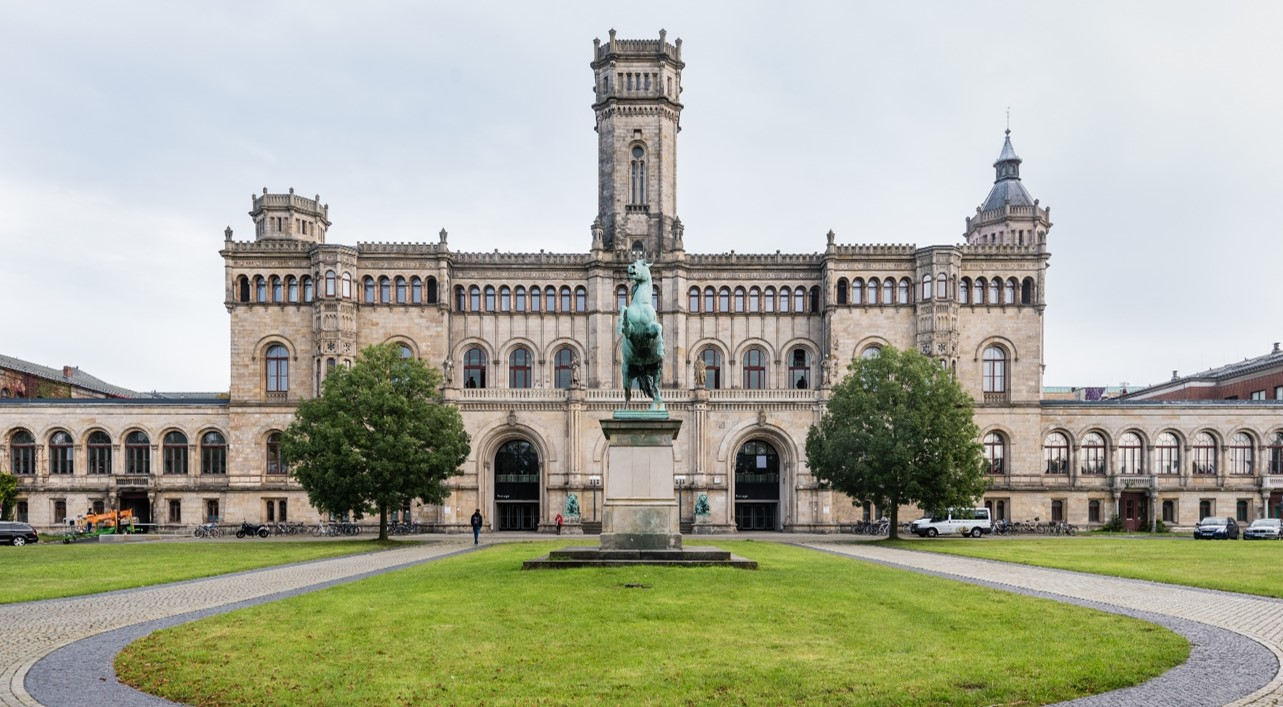
\includegraphics[width=0.65\textwidth]{figures/luh_default_presentation_title_image.jpg}}

% Title page: luhstyle
% \setbeamertemplate{title page}[luhstyle]
% % Add optional title image here
% \addtitlepageimage{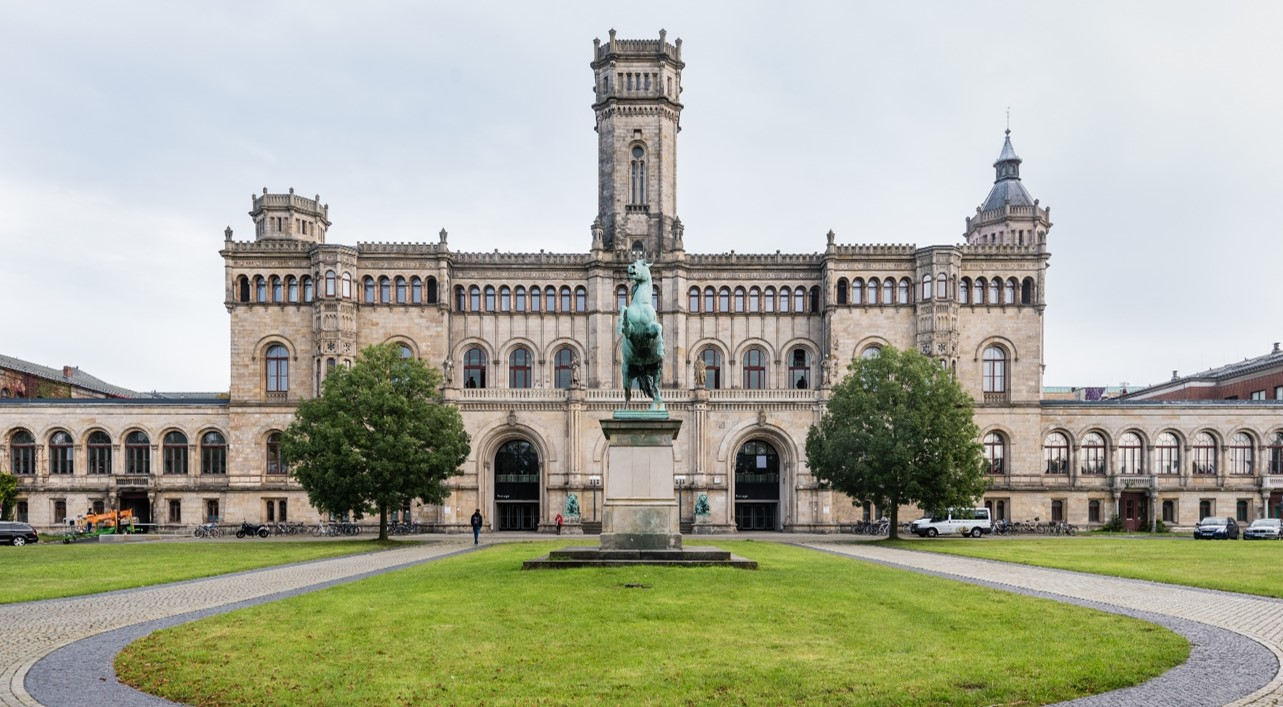
\includegraphics[width=0.75\textwidth]{figures/luh_default_presentation_title_image.jpg}}

\author[Abedjan \& Lindauer]{Ziawasch Abedjan \& Marius Lindauer\\[1em]
	
\includegraphics[height=\logoheight]{../latex_main/figures/luh_logo_rgb_0_80_155.pdf}\qquad
	
\includegraphics[height=\logoheight]{../latex_main/figures/DBIS_Kurzlogo.png}\qquad

\includegraphics[height=\logoheight]{../latex_main/figures/TNT_darkv4}\qquad

\includegraphics[height=\logoheight]{../latex_main/figures/L3S.jpg}	}
\date{Summer Term 2022; \hspace{0.5em} {
\includegraphics[height=1.5em]{../latex_main/figures/Cc-by-nc-sa_icon.svg.png}}; based on \href{https://ds100.org/fa21/}{[DS100]}
}


%%% Custom Packages
%----------------------------------------------------------------------
% Create dummy content
\usepackage{blindtext}

% Adds a frame with the current page layout. Just call \layout inside of a frame.
\usepackage{layout}


%%% Macros
%\renewcommand{\vec}[1]{\mathbf{#1}}
% \usepackage{bm}
%\let\vecb\bm

\title[Gradient-Boosting Trees]{DS: Decision Trees}
\subtitle{Gradient-Boosting Trees}

\graphicspath{ {./figure_tree/} }
%\institute{}


\begin{document}
	
	\maketitle
	\begin{frame}[c]{Gradient-Boosting Trees}

    \begin{itemize}
        \item The most popular model in Kaggle Competitions\footnote{\url{https://www.kaggle.com/}} for tabular data is XGBoost
        \begin{itemize}
            \item XGBoost = Extreme Gradient Boosted Trees
        \end{itemize}
        \smallskip
        \item Main Idea:
        \begin{itemize}
            \item Random Forest build an ensemble of independent decision trees
            \item Instead of independent trees, try to improve the first trees with the following trees
            \item Each additional tree should directly contribute to improve the ensemble (not only by chance!)
        \end{itemize}
    \end{itemize}

	\end{frame}
	
	\begin{frame}[c]{Correcting Predictions}

    \vspace{-1em}
    \begin{itemize}
        \item Let's assume that we fitted $m$ trees $\hat{F}_m$ already
        \item All of these together provide a prediction for a given input:
        $$ \hat{F}_m(\bm{x}_i) = \hat{y}_i $$
        \smallskip
        \item The model will now be off from the true label $y_i$ to a certain degree
        $$e_i = y_i - \hat{F}_m(\bm{x}_i)$$
        \item Remember: residuals!
        \smallskip
        \item Can we add a model that correct our ensemble $\hat{F}_m$ in the directions of the residuals by adding another model $\hat{f}_{m+1}$?
        $$ \hat{f}_{m+1} :=  y_i - \hat{F}_m(\bm{x}_i)$$ 
        \item if $ \hat{f}_{m+1}$ could perfectly learn the residuals, $\hat{f}_{m+1} +  \hat{F}_m(\bm{x}_i)$ would be a perfect model
    \end{itemize}

	\end{frame}
	
	\begin{frame}[c]{Learning how to boost}

    \vspace{-1em}
    \begin{itemize}
        \item Coming back to the idea of ensembles $F$ (with $M$ base models) by weighting $\gamma$ each model:
        
        $$ \hat{F}(\bm{x}) = \sum_{m=1}^{M} \gamma_m \hat{f}_m(\bm{x}) + c $$
        \item Let's start with fitting a first constant base model on all training data
        $$F_0 \in \argmin_{\gamma} \sum \mathcal{L}(y_i, \gamma) $$
        \item Extend the ensemble by a base model correcting for the residuals -- recursive definition!
        
        $$ F_m (\bm{x}) = F_{m-1}(\bm{x}) + \argmin_{h_m} \left[ \gamma_m \sum_i \mathcal{L}(y_i, F_{m-1}(\bm{x}_i) + f_m(\bm{x}_i)) \right] $$
    \end{itemize}

	\end{frame}
	
	\begin{frame}[c]{Learning how to boost (cont'd)}

    \vspace{-1em}
    $$ F_m (\bm{x}) = F_{m-1}(\bm{x}) + \argmin_{h_m} \left[ \sum_i \mathcal{L}(y_i, F_{m-1}(\bm{x}_i) + f_m(\bm{x}_i)) \right] $$
    \begin{itemize}
        \item[$\leadsto$] that would be an infeasible optimization problem
        \item[$\leadsto$] take a step in the steepest direction (steepest descent) of this minimization problem:
        $$ F_m(x) = F_{m-1}(\bm{x}) - \gamma \sum_i \nabla_{F_{m-1}} \mathcal{L}(y_i, F_{m-1}(\bm{x_i})) $$
        \item where $\gamma$ is the step length
    \end{itemize}

	\end{frame}
	
	\begin{frame}[c]{Practical Considerations}

    \begin{itemize}
        \item Base models should be very shallow models, e.g,, decisions trees with a single split
        \smallskip
        \item Learning rate $\gamma_m$ decides how many trees you need to change the predictions
        \begin{itemize}
            \item too large $\gamma$ will lead to unstable learning
            \item too small $\gamma$ will lead to very slow learning and large models
            \item[$\leadsto$] often between $0.3$ and $0.1$ $\leadsto$ better to tune it explicitly (e.g., with Bayesian Optimization)
        \end{itemize}
        \smallskip
        \item One of the most robust and well-performing ML models for tabular data
        \begin{itemize}
            \item Nevertheless, good feature engineering and preprocessing can be crucial
        \end{itemize}
        \smallskip
        \item XGBoost is one of the most well-known libraries for gradient-boosting trees:\\ \url{https://xgboost.readthedocs.io/en/stable/index.html}
    \end{itemize}

	\end{frame}
	
	
\end{document}